\documentclass{standalone}
\usepackage{tikz}
\usepackage{tikz-feynman} % Paquete para diagramas de Feynman
\begin{document}

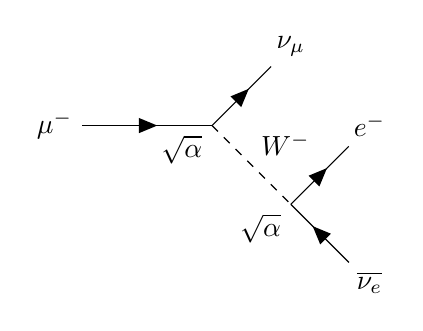
\begin{tikzpicture}
    \begin{feynman}
        % Nodos de partículas
        \vertex (i1) at (-1,1) {\(\mu^{-}\)};
        \vertex[label=below left: {$\sqrt{\alpha}$}] (v1) at (1,1);
        \vertex[label=below left: {$\sqrt{\alpha}$}] (v2) at (2,0);
        \vertex (v3) at (3,1) {$e^-$};
        \vertex (i2) at (2,2) {\(\nu_\mu\)};
        \vertex (v4) at (3,-1) {$\overline{\nu_e}$};
        
        % Diagramas de líneas
        \diagram* {
            (i1) -- [fermion] (v1), % Línea del electrón
            (v1) --[dashed, edge label = $W^-$] (v2), % Línea del electrón desviado
            (v1) -- [fermion] (i2),  % Línea del fotón después de la interacción
            (v2) -- [fermion] (v3),
            (v4) -- [fermion] (v2),
        };
    \end{feynman}
\end{tikzpicture}

\end{document}
